{\color{gray}\hrule}
\begin{center}
\section{Technical Approach}
\textbf{bla bla }
\end{center}
{\color{gray}\hrule}


\begin{multicols}{2}
In order to get across the inner workings of each module we will separate this section into subsections related to each one.

\subsection{Pre-processing}
As the objective of the system is to be adaptable to dirty and noisy input images, in the pre-processing phase great care should be taken to clean such inputs. As such the pre-processing module performs different methods of input refinement.

A first denoising pass is performed utilizing the bilateral filter, after which the image goes through a light adjustment procedure which entails contrast stretching.

After these operations we perform the background removal. This is because we thought that a potential point of improvement within the virtual try-on pipeline could be the removal of the background before going deeper into the network as the background information may hinder the performance the subsequent modules. To perform such a task we are looking and comparing multiple already existing solutions such as:
\begin{itemize}
\item U-Net: fine-tuning a pre-trained U-Net model using the Tik-Tok dataset;
\item Detectron2: fine-tuning on Dress-Code the Detectron2 segmentation module released by Facebook.
\end{itemize}

We will compare the results and choose the best one according to state-of-the-art evaluation metrics (DICE etc...).



\subsection{Person representation}
This module deals with the semantic segmentation of the subject and their keypoints extraction, which will be used to as features for the warping module.

Regarding the segmentation problem we have, as of now, identified the Detectron2 segmentation module as the main candidate to solve it.

Instead, for the keypoint extraction problem we are comparing the DensePose module (from Detectron2) and the OpenPose module.




\subsection{Warping module}
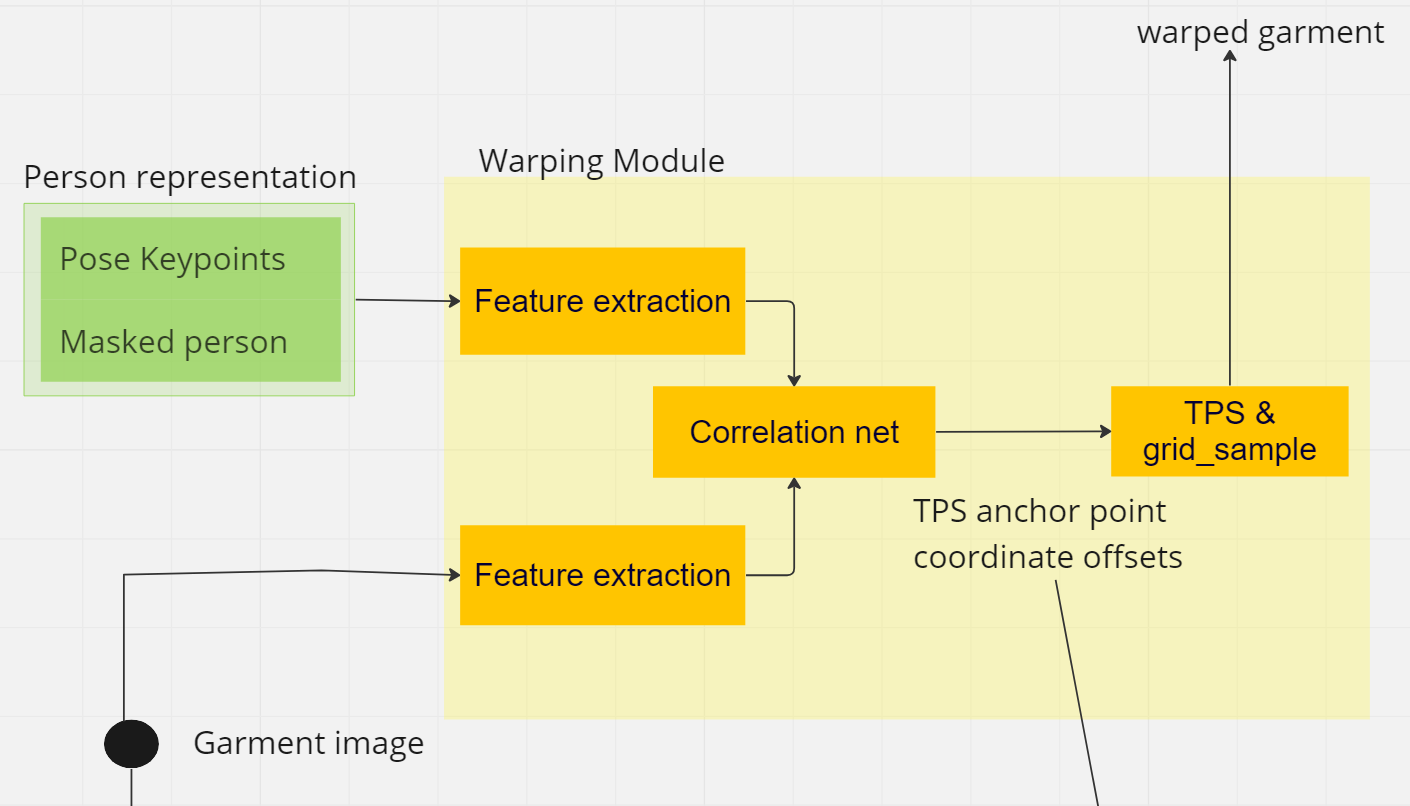
\includegraphics[scale=0.4]{warping_module_schema}

The warping module takes as inputs the person representation feature vector and the garment image and, based on the keypoints and the segmantation mask, it warps the garment fitting it to the body shape of the subject.

The output is the set of the TPS parameters, which are used to geometrically transform the clothing item.



\subsection{Generative module}





\end{multicols}